%*******************************************
\section{App Teaching Content}
%*******************************************

In this chapter we describe and elaborate on different teaching and learning contents which can potentially be communicated to the user.
 At the same time we reason our decision whether to communicate the specific content or not.


\subsection{E-Mail Spoofing}
%...........................................
According to a study by DIVSI~\cite{divsi2012divsi}, 85\% of the Internet users utilize e-mails for communication but only 14\% have concerns regarding e-mail security.
This misconception is also reflected in our phishing survey (cf. \autoref{s:survey}).
This is a problem because in contrast to public belief e-mail is not secured against fraud. There are three main facts that need to be delivered to the user:
\begin{description}[leftmargin=0cm]
	\item[From Field:] A major misbelief is that an e-mail's from-field is in some way secured.
	In reality it must be considered a plaintext field.
	The problem is that most modern e-mail clients hide this fact away from the user.
	Therefore, we have to explain to the user that anyone can send e-mails from any from address. 
	\item[E-Mail Content:] We also have to show the user that the content of the e-mail is totally in the control of the sender.
	Nobody prevents the attacker from sending e-mails that look exactly like the ones sent out by a legitimate sender.
	\item[Links in E-Mails:] The third aspect that most users are not aware of is that e-mail links or links in general could point to any page. 
	This means that the link does not necessarily lead to the denoted URL.
\end{description}
The above mentioned learning contents are intended to increase the user's security awareness.
In \autoref{s:app_design} we describe how exactly we achieve to communicate these teaching contents to the user.

\subsection{Smartphone Limitations}
%...........................................
As already discussed in \autoref{s:antiphishing_on_smartphone} smartphones have several limitations, such as the small screen size. 
This section deals with the detection of phishing on the smartphone and the related limitations.
More particularly, we will briefly explain in which ways URLs can be checked with the smartphone and what kind of problems these operations raise.
Based on this we decide whether to communicate this kind of URL checking to the user or not.

\begin{description}[leftmargin=0cm]
	\item[Invisible Address Bar:] As discussed in \autoref{s:antiphishing_on_smartphone}, due to the lack of space most of the smartphone browsers hide the address bar, i.e. the URL,~\cite{amrutkar2012measuring} and use this expanded space for the web content (cf. \autoref{fig:screenshot_addr_bar_hidden}). This is an issue which can and should be solved on a technical basis. In fact, some versions of the Android browser already fix this by always displaying the address bar. As long as this is not applied to a majority of active Android systems, this must be communicated to the user because the address bar contains the important information of a website's URL.
Most of the users will probably know how they can access the address bar of their browser.
However, for those who might not know how to deal with that an introduction is inevitable.
\begin{figure}
\centering
\subfigure[Address bar hidden]{\label{fig:screenshot_addr_bar_hidden}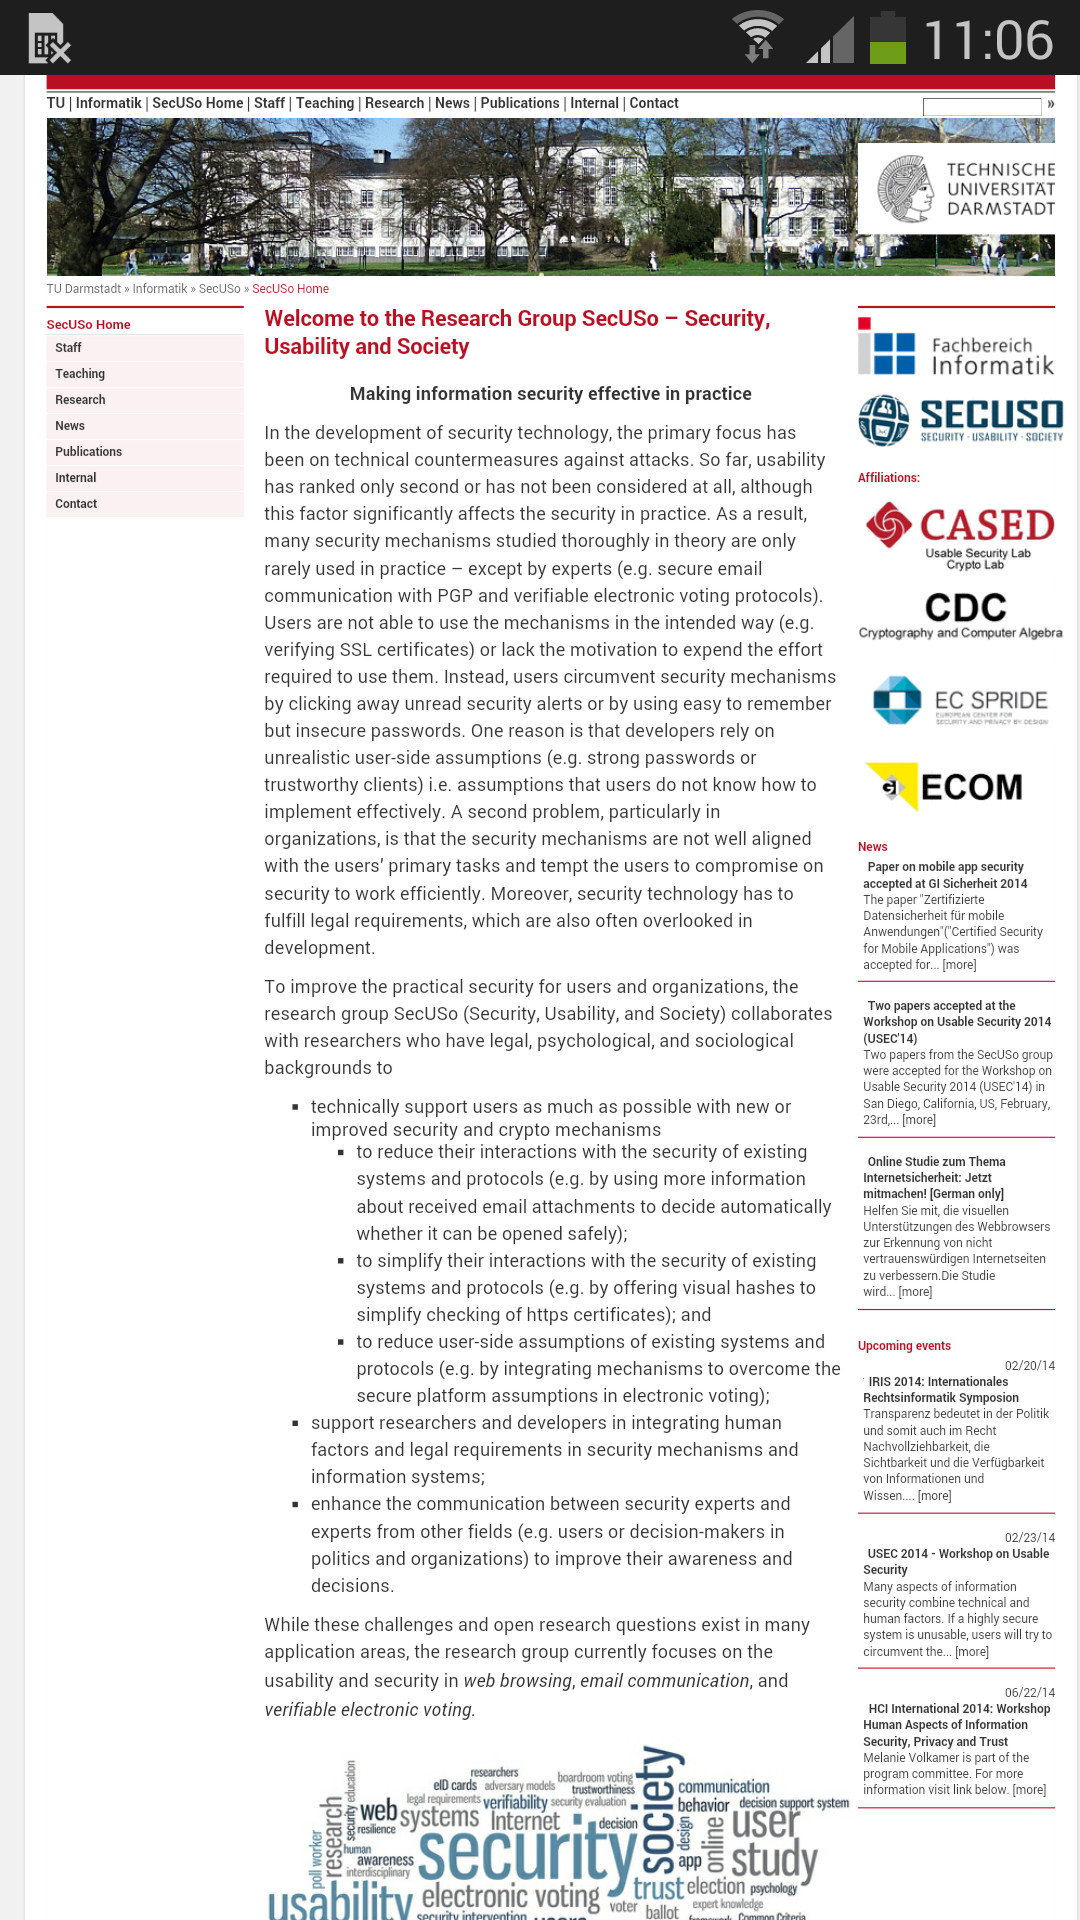
\includegraphics[width=0.45\textwidth]{Screenshot_addressbar_hidden.png}}
\subfigure[Address bar visible with padlock]{\label{fig:screenshot_addr_bar_visible}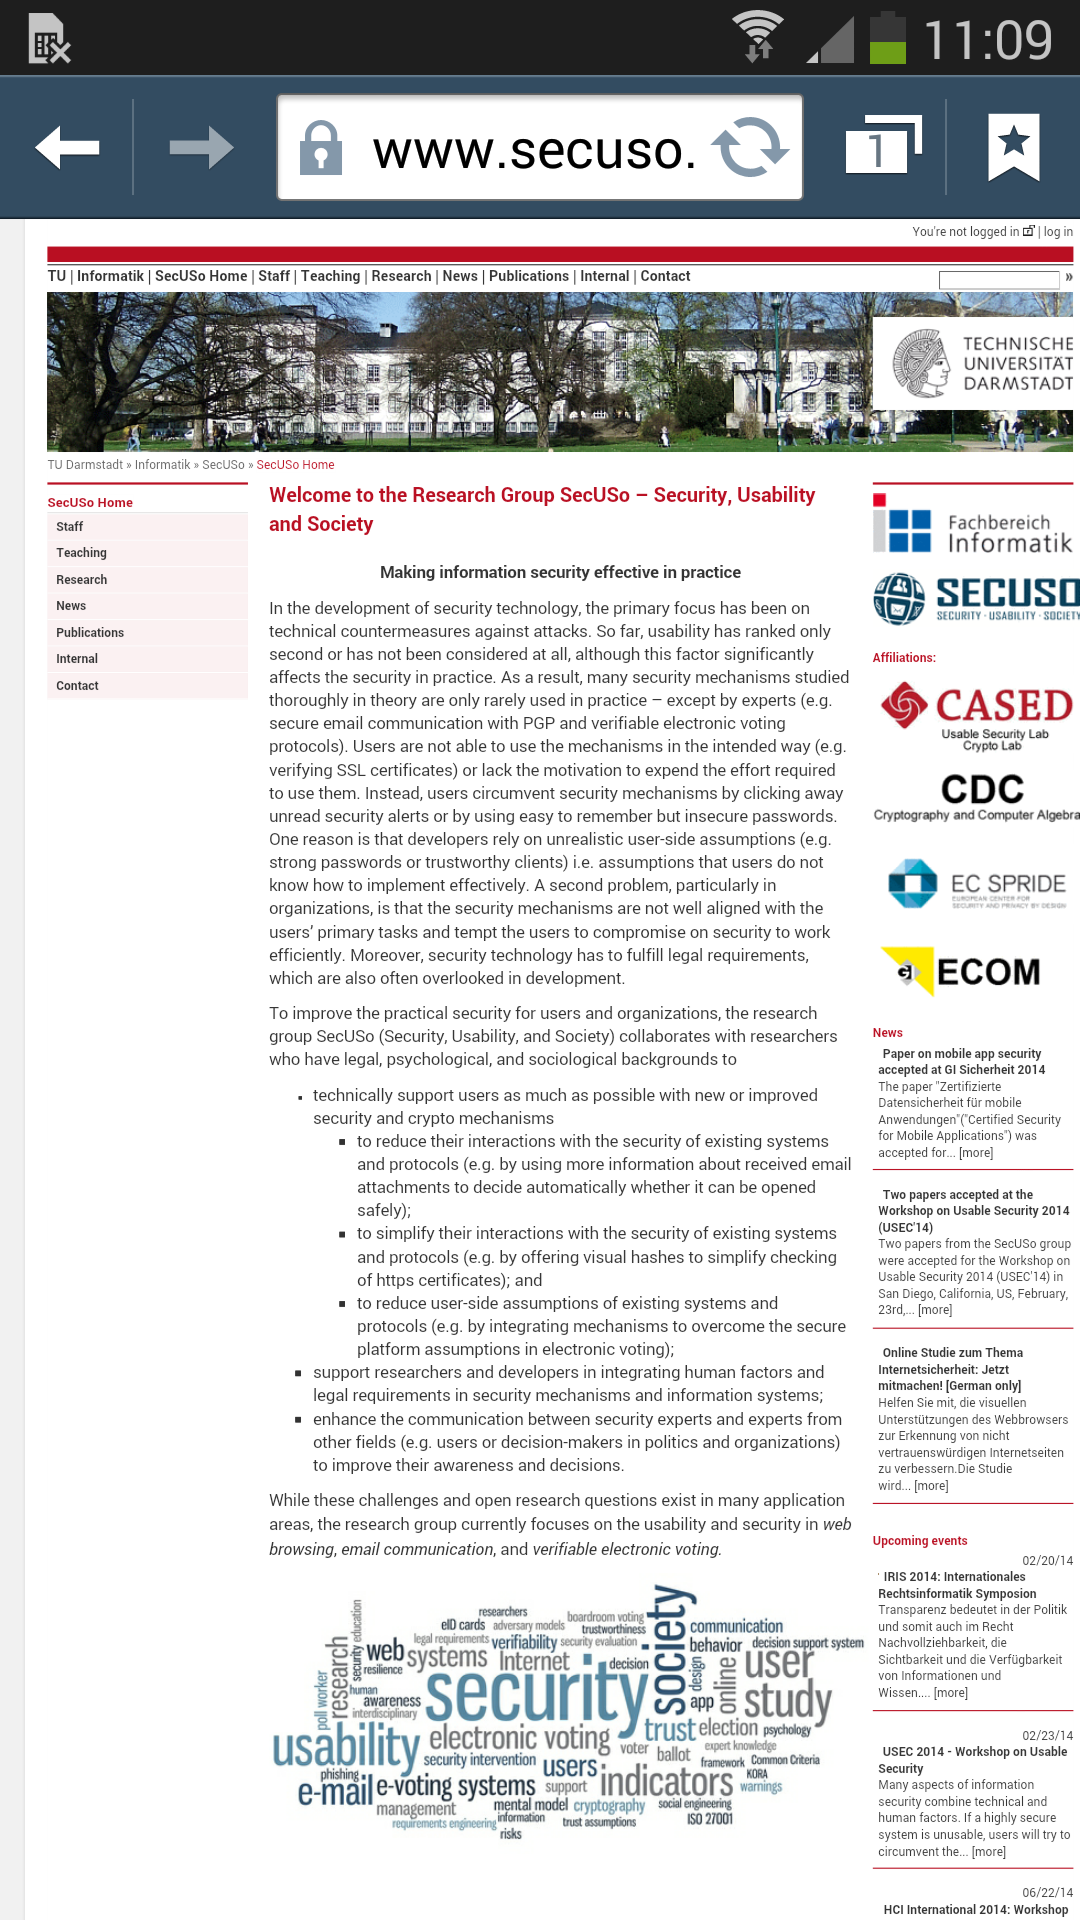
\includegraphics[width=0.45\textwidth]{Screenshot_addressbar_visible_padlock.png}}
\caption{Visibility of the address bar}
\label{fig:screenshot_addr_bar}
\end{figure}
	\item[Analyze Complete URL Via Address Bar:] Finding the address bar will not suffice for a reasonable URL analysis. 
Here again, the small screen size makes it is impossible to view the complete URL without any further action (cf. \autoref{fig:screenshot_addr_bar_visible})).
Specifically, it is necessary to first tap the URL address text and then scroll the pointer to the left and right for the URL analysis.
Without learning these steps a reliable URL checking is not possible. 
Therefore, these steps have to be communicated to the user.

	\item[Analyze URL After Click:] In \autoref{s:coverage} we extensively discussed the advantages and disadvantages of the URL analysis before as well as after clicking on a link.
The reasons why we decided to go for an after click URL analysis can be consulted in that section.
Hence, functionalities or workarounds related to showing the destination URL before clicking on a link will not be communicated to the user.
Instead we focus on the URL analysis directly in the browser.
\end{description}

\subsection{Structure of a URL}
\label{s:url_structure}
The URL is a complex construct. 
In order to correctly analyze a URL and decide whether it is spoofed or not it is necessary to understand its structure. 
Therefore, the users must achieve the essential capability of parsing a URL appropriately.
An attacker uses brands which are familiar to the user in any part of a URL in order to deceive him. 
Thus, especially the identification of the domain in a given URL is a key aspect which must be covered extensively within the app. 
We will teach the user about the most important parts of a URL, the protocol (HTTP vs. HTTPS), the host with its domain and the path.
We do not distinguish the directory, filename or query parameters of the URL path because this part is rather irrelevant for the detection of phishing.
By contracting these elements we can avoid discouraging and overwhelming users with details they do not need.

\subsection{Phishing URLs}
%===========================================
As aforementioned, we focus on teaching the user how to analyze a given URL and to decide whether it belongs to a legitimate or illegitimate website.
 In order to distinguish legitimate URLs from phishing URLs it is necessary to analyze existent phishing URLs regarding the way they are spoofed in order to deceive the users.
 For the analysis of phishing URLs we chose the database of PhishTank~\cite{phishtank}.
PhishTank is a free community site where people can submit, verify and view phishing data.
 It provides an API which makes all PhishTank data accessible.
 Organizations such as Yahoo, Kaspersky Lab and Mcafee use the data submitted by PhishTank. A further reason to choose PhishTank as our phishing URL database was that a contact at Kaspersky Lab himself recommended to make use of it for our URL analysis.
 For the phishing URL analysis we drew on the URL categories identified by the authors of Anti-Phishing Phil~\cite{sheng2007antiphishingphil} as our baseline.
 These include IP address URLs, subdomain URLs as well as similar and deceptive domain URLs.
 Subsequently, we went through the PhishTank URLs and tried to assign them to one of these categories.
 When no category suited the URL to be assigned, we generated a new category, to which the URL could then be assigned to.
 In addition, we found various categories mentioned in literature, which we also included to our categories, even if we could not find any explicit example URLs in the PhishTank database.
 In the following we explain the identified URL categories.
%...........................................
\subsubsection{Phishing URL Categorization}
%...........................................
\label{s:url_categories}
URLs are complex and many users do not know how exactly they have to be interpreted.
 For example, users can be convinced of the authenticity of URL when it contains the brand name anywhere.
 Phishers exploit this lack of knowledge in different ways.
 In the following we present the identified categories of spoofing attacks on URLs. 
 All spoofing attacks are covered by the app unless noted otherwise.

\begin{description}[leftmargin=0cm]
	\item[Subdomains:] Phishers make use of subdomains which are very similar or even identical to the domains of the targeted institutions.
 For example, they register a domain  ``xyz.com'' and use ``paypal'' in their subdomain, resulting in a URL such as ``http://www.paypal.xyz.com/webapps/''.
 This makes the users believe that they are on a legitimate website.

	\item[IP Addresses:] Sometimes phishers do not even bother registering any domain at all.
 In this case, the host area of the URL contains an IP address.

	\item[Nonsense Domains:] We frequently encountered URLs which had registered random names or strings as their domain.
 The domain names ranged from random letters to domain names like ``marketstreetchippy.com''. In order to deceive the users some of these URLs contained a well-known brand name in other parts of the URL.
Yet, there were a number of examples where this was not the case, i.e. without viewing the content of the website one would have no idea where the URL points to.

	\item[Trustworthy, but Unrelated Domains:] Some URLs are very well-crafted.
 When reading them they appear meaningful and trustworthy.
 This is particularly accomplished by registering domain names which sound reliable, for example, ``account-information.com'', ``secure-login.de'', or ``security-update.com''. If the URL additionally contains the brand name of the targeted institution somewhere in the URL the user can be easily deceived.

	\item[Similar and Deceptive Domains:] Another possibility to fool users with a spoofed URL is to use URLs which look like the original ones, but have a slight difference.
 For example, phishers register domains which resemble the targeted domain, but have a typo.
 To spoof ``paypal.com'', for instance, the attacker might register ``paypel.com''. Another approach is to use a modification of the original domain.
 The modified domain contains the brand name in some form.
 For example, ``facebook-login.com'' can be registered in order to fake ``facebook.com''. Finally, the attacker can scramble letters of the original domain, which can be very hard to detect at first sight.

	\item[Homograph Attacks:] The homograph attack exploits character resemblance.
 Here, characters are replaced by other characters which look very similar to the replaced one.
 For example, an attacker might replace a ``w'' within a genuine domain with ``vv'' and register it.
 An even more advanced way is to replace characters of the genuine domain with characters from other character sets, such as Cyrillic languages, where the characters will look almost identical~\cite{gabrilovich2002homograph}. The latter case is indistinguishable for the human eye in many cases and is partially a technical issue.
Here, browser vendors should be encouraged to indicate when international characters are contained in a URL.
 For this reason, only cases that are distinguishable by the human eye are covered by the educational app.

% DAS WAS DER USER NICHT SEHEN KANN WIRD NATÜRLICH AUCH NICHT GECOVERED WERDEN KÖNNEN
	\item[Tiny URLs:] A tiny URL service is used to convert a long URL into a short one.
 Due to their shortness tiny URLs are very comfortable to use and easy-to-type.
 There seemed to be a trend of using tiny URLs for phishing in 2009, in particular in instant messaging services~\cite{tinyurlpcworld}.
 Tiny URLs usually do not give a hint about the target website and users do not tend to be suspicious about receiving such links from a ``friend'' what made the use of them for the purpose of phishing quite popular. Tiny URLs redirect the shortened URL to the actual one.
 As we consider the ``analyze URL after click'' scenario for the user education, there is no need of the tiny URL to be covered by the app.

		\item[Cloaked URLs:] Other phishers integrate an ``@'' into the URL so that domain names become difficult to understand and the actual destination of a link becomes ``cloaked''~\cite{alnajim2009fighting}. For example, the URL ``http://paypal.com@google.com/'' is redirected to ``http://google.com''. 
As we consider the ``analyze URL after click'' scenario for the user education, there is no need of the cloaked URL to be covered by the app.

\end{description}

%...........................................
\subsubsection{Problems with URLs}
%...........................................
\label{s:problems_with_URLs}
There arise two major problems with the detection of phishing attacks based on the URL.


\begin{enumerate}
	\item Some legitimate URLs feature characteristics of phishing URLs.
	\item We cannot assure that the users know all website vendors of our URLs (whether legitimate or phish).
\end{enumerate}
This section elaborates on these problems and outlines how we approach to handle these issues.

\begin{description}[leftmargin=0cm]
	\item[Legitimate, but Fraudulent Looking URLs:] 
We wanted to find out to what extent our determined phishing URL categories from \autoref{s:url_categories} apply to authentic websites.
For this purpose, we browsed the web and looked at the top 50 banks~\cite{bankrank} and top 50 online shops~\cite{onlineshoprank} in Germany. 
While surfing on these websites we recognized that it occasionally happens that a legitimate URL features the characteristic of a phishing URL. 
This is particularly the case for the category of similar and deceptive domains. 
There exist sites of vendors which make use of similar domains, instead of never changing the domain and using, for example, subdomains. 
An example is the website of the Commerzbank. 
When surfing on Commerzbank's website the domain is ``commerzbank.de''. 
Once the user is on the online banking part of the website the domain changes to ``commerzbanking.de''. 
The same happens on the PayPal website. 
The regular website features the domain ``paypal.com''.
However, paypal also has a site, where the domain is ``paypal-viewpoints.com''.
By our definition, ``commerzbanking.de'' and  ``paypal-viewpoints.com'' contain indications of a phishing website.
We decided to address this problem by adding a section of final remarks to the app. 
In this section we tell the user that there might be legitimate domains which are similar to domains they are familiar with and that these not necessarily are phishes. 
We still strongly recommend the user to directly contact the vendor before submitting data to such websites. 
The reason why we do not address this problem in the according level is that we do not want to degrade the user's attention by telling him that similar domains might still be legitimate. 
We do not consider it an issue that the user is told about this later in the app, since it is better to reject a legitimate URL than trusting a phishing URL. 

\item[Unknown Website Vendors:] Despite our efforts of mainly making use of URLs from widely known website vendors there is still the possibility that a user does not know all vendors and thus the respective URL. 
One approach to address this problem is that the user has to indicate which websites he knows with the aid of a long list of check boxes, for example. 
We decided against this approach for two reasons: 
First, if a user only knows a few website vendors, the list of available URLs to be drawn from would be quite short. 
And thus the game experience will degrade significantly. 
Second, and more importantly, we cannot expect the users to go through a large list of vendors and let them decide whether they know them or not. 
This kind of configuration would substantially decrease the usability and acceptance of our app. 
Currently, we have to let the user learn new vendors. 
By making mistakes and/or giving correct answers to unknown URLs, i.e. domains, the user will likely gain experience and learn whether a given domain is legitimate or not. 
For future work one might consider to add an ``I don't know'' button to the options a user has during a challenge in a level of the app.
In this case the user could be explained whether it is a phish or not and why it is so.
This option should be punished in some way in order to prevent the user from picking only easy URLs for his answers.
\end{description}


\subsection{General Recommended Behavior}
There are general hints and tips for Internet users which can be helpful to protect oneself against phishing.
The user should be informed about these general recommendations at some point.
These aspects are explained in the following.

\begin{description}[leftmargin=0cm]
	\item[Data Entry Via HTTPS:] 	When the user enters data via HTTP there are basically two problems.
	First, the user cannot be sure that he actually is communicating with the website it claims to be.
Second, even if the user actually communicates with the intended communication partner there still might be an attacker wiretapping the communication.
Therefore, data that is sent via plain HTTP is considered lost. 
	This teaching content is covered by our app (cf. \autoref{s:knowledgetransferperlevel}).	
	\item[Do Not Download Attachments:] Many users download or even open files that they receive via e-mail rather unchecked.
	This is related to the problem that they trust the from field of the e-mail.
	It is crucial to tell them that downloading or opening an unknown file might infect their system.
	As discussed in \autoref{s:assumptions} we assume that users are not tricked into downloading malicious software.
This aspect remains open for further research.
	\item[Data Economy:] The goal of this app is to prevent the users' data from being phished.
	A further step towards this goal is to teach the user to enter sensitive data as rarely as possible.
	The idea behind this is that websites, including but not limited to, phishing websites, might exploit user data. 
	For now we put our focus on the detection of phishing URLs.
The aspect of re-thinking what data to provide to what kind of service remains an issue to be targeted in future work.
\end{description}

%...........................................
\subsection{Browser Security Indicators}
%...........................................
As a matter of fact, there is a major lack of mobile browser security indicators~\cite{amrutkar2012measuring,trusteer2011}. 
Yet, there exist some, for example, the padlock for the usage of HTTPS.
Such signals have the potential to provide relevant information to the user which we would have liked to inform them about.
However, besides the lack of such hints there is also the problem of inconsistencies among the mobile as well as desktop browsers.
Ultimately, our decision was not to tell anything about these security indicators, as the inconsistencies are too significant even among the standard browser, depending on the device and Android version it is installed on.
\begin{description}[leftmargin=0cm]
		\item[HTTPS Padlock] All Android standard browsers on various devices we examined have a padlock in the address bar on SSL secured pages (cf. \autoref{fig:screenshot_addr_bar_visible}).
Also, one should consider that there are illegitimate as well as legitimate websites where a padlock is part of the web content. 
Therefore, it is important to teach the users to look for the padlock in the browser, not in the content, to verify that the site they visit is SSL secured, when they enter confidential data.
However, some browsers additionally make use of so called favicons, i.e. small website icons.
The danger of using such a favicon is that a phisher could use the image of a padlock in order to deceive the user~\cite{trusteer2011}.
Moreover, the padlock with/without favicon combinations appear in different ways. 
While a part of the stock browsers installed on various devices and Android versions we examined only feature a padlock in case of HTTPS websites and no favicon at all, others always display favicons. 
In the latter case, if HTTPS is used the padlock is either positioned right next to the favicon or overlaps it.
Due to the variety of possible combinations as well as the deception potential in combination with favicons we decided not to tell the user about the padlock.
		\item[Touch Padlock] Touching the padlock of an SSL secured website on some browsers leads to an alert dialog with information about the website. 
One part of this information is the complete URL of the website the user is currently on.
In this case, it would become possible to view and analyze the complete URL without tapping the address bar and scrolling to the left and right.
For \textit{some} browsers which additionally display favicons, the above described feature is always applicable.
That means, the alert dialog with the complete URL can also be consulted on websites which do not use HTTPS.
Yet, there are also browsers where neither clicking on a padlock nor on a favicon is possible.
Hence, we will stick to our approach, where the user is explained how to analyze the URL directly in the address bar.
		\item[Certificate Verification]Tapping on the padlock icon in some browsers results in an alert dialog where the user can select to view the certificate details (``show certificate'').
As already stated, the padlock feature is not consistent over the various devices and browser versions.
Hence, in these cases a validation of the certificate is not possible as well.
Therefore, this is an aspect which is not covered by our app.

\end{description}

%...........................................


%...........................................
\subsection{Summary}
%...........................................

This section briefly lists the above described learning contents which will be addressed by our app.
In the following section we precisely explain how the learning contents are reflected in our app and provide further insights to our app design.

\begin{enumerate}
	\item E-mail spoofing 
	\begin{enumerate}
		\item Do not trust the sender
		\item Do not trust the content
		\item Target URL of a link is not necessarily the displayed one
	\end{enumerate}
	\item Invisible address bar
	\begin{enumerate}
		\item Access address bar
		\item View complete URL
	\end{enumerate}
	\item Structure of a URL
	\item Phishing URL categories
	\begin{enumerate}
		\item Subdomain attack
		\item IP address attack
		\item Nonsense domain
		\item Trustworthy sounding, but unrelated domain
		\item Similar and deceptive domain
		\item Homograph attack
	\end{enumerate}
	\item General recommended behavior
	\begin{enumerate}
		\item Data entry via HTTPS only
	\end{enumerate}
	
\end{enumerate}
